%\documentclass[12pt,a4paper]{report}
%\usepackage[utf8]{inputenc}
%\usepackage[english]{babel}
%\usepackage{amsmath}
%\usepackage{amsfonts}
%\usepackage{amssymb}
%\usepackage{graphicx}
%\usepackage{eurosym}
%\usepackage[left=2cm,right=2cm,top=2cm,bottom=2cm]{geometry}
%\usepackage{wrapfig}
%\usepackage{mathdots}
%\usepackage{caption}
%\usepackage{cite}
%\usepackage{mathrsfs}
%\usepackage{float}
%\author{Oscar Fuentes Muñoz}
%\title{Data Link Layer Protocol}
%\begin{document}
%\maketitle
%\tableofcontents
%\listoffigures
%\listoftables
%\chapter{PolarOrbit}

\subsection{Introduction}
Polar Orbits are commonly used for a broad variety of applications. The most significant and clearest example is the GPS (Global Positioning System) constellation. 
\\
\\
The GPS Constellation
\\
The GPS is a constellation property of the U.S. It provides positioning, navigation and timing. The constellation was designed with a 24-slot arrangement to ensure a visibility of at least four satellites from any point on the planet. Nowadays the constellation has expanded to a total operative number of 27-slot since June 2011. Some characteristic parameters of the satellites are the following:

\begin{itemize}
\item Orbit: MEO
\item Height = 20,200 km;
\item Lifetime = 12.5 years;
\item Cost = 166 million USD;
\end{itemize}

\begin{figure}[H]
\begin{center}
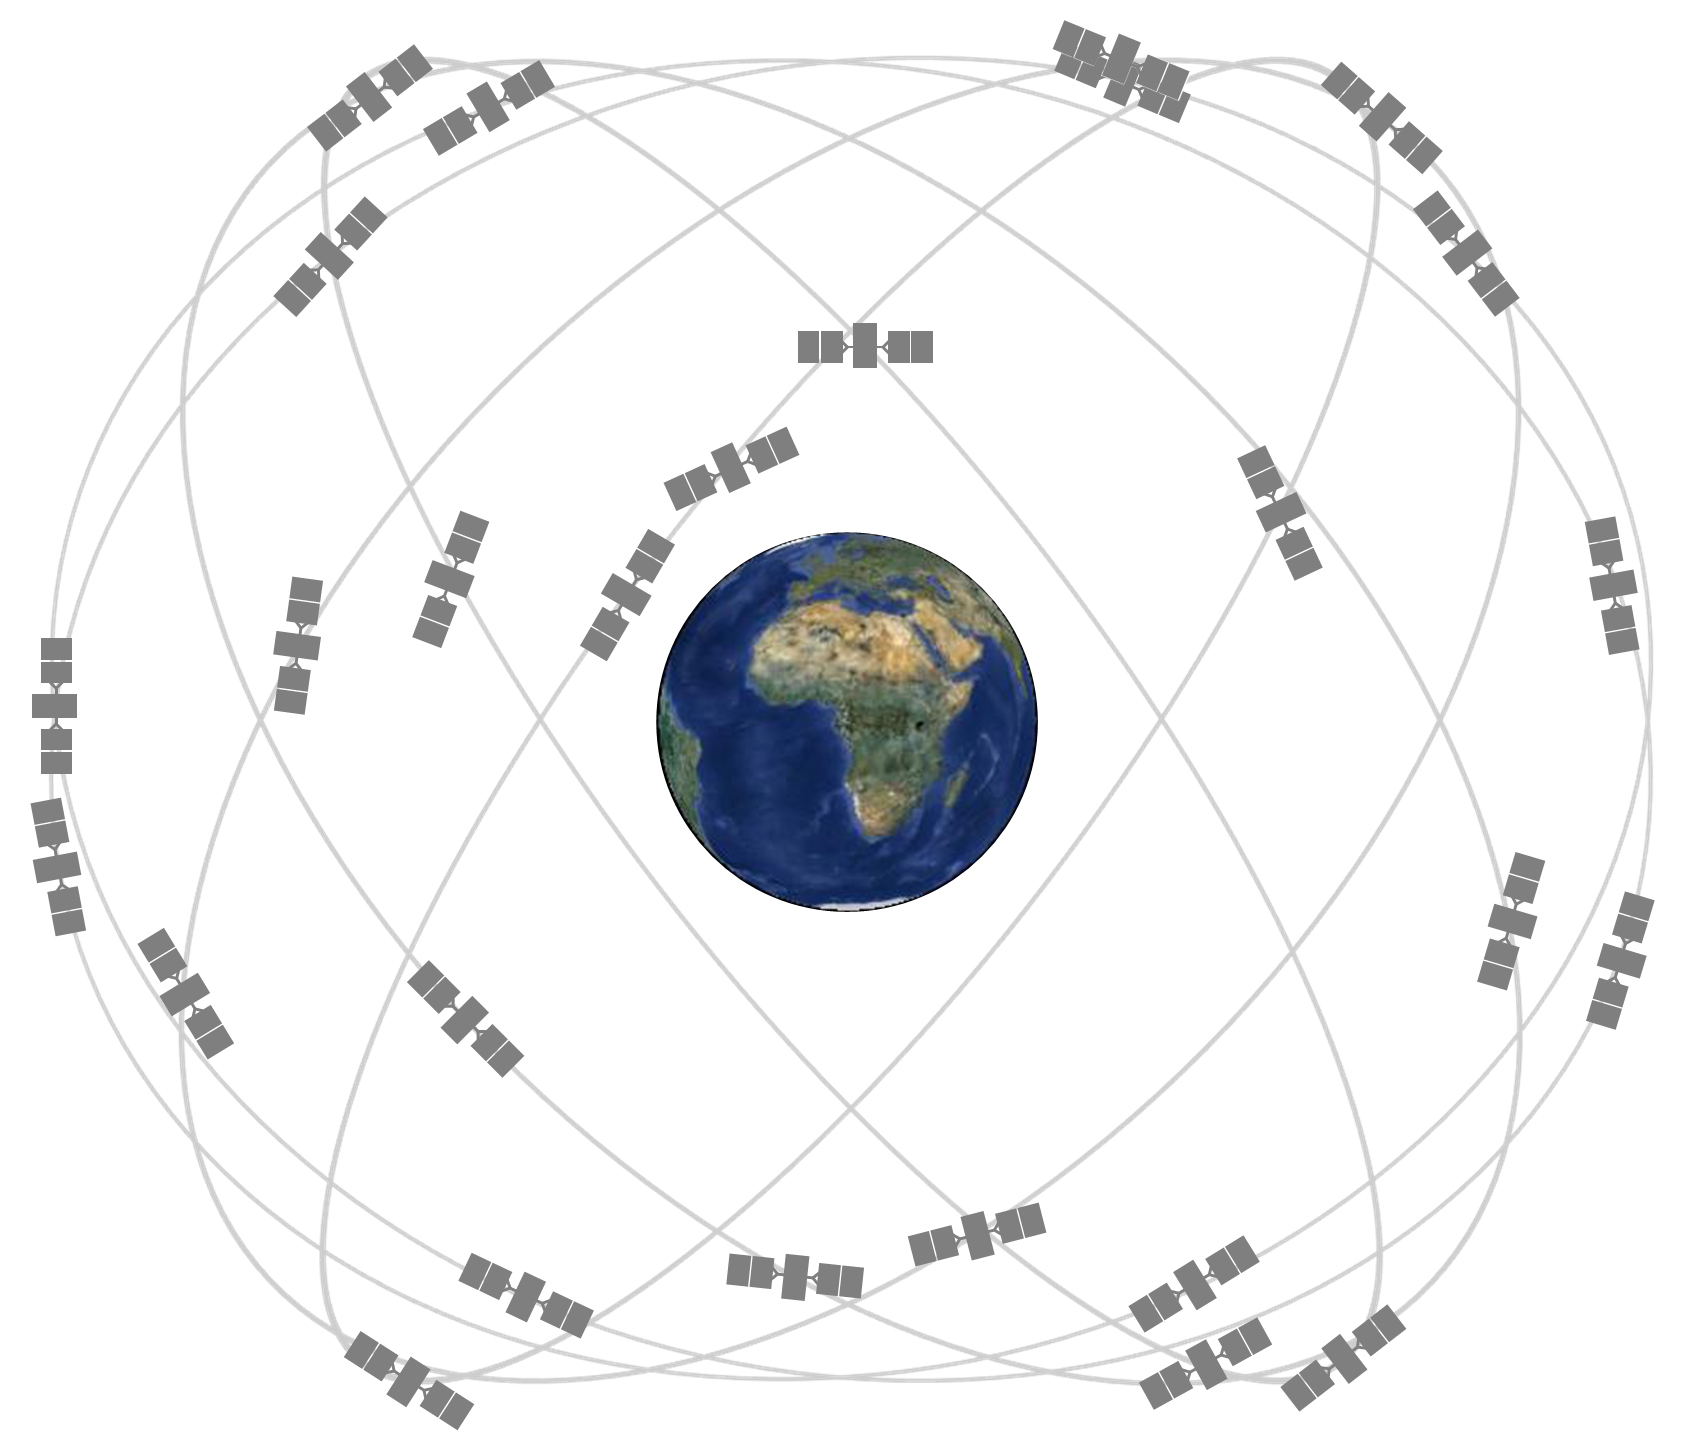
\includegraphics[scale=0.2]{PolarOrbits/GPSconstellation.jpg}
\caption{Distribution of the expanded 24-slot GPS constellation.}
\end{center}
\end{figure}

\subsection{General Configuration}
The Polar Orbits configuration consists in the distribution of plains with inclination equal to 90 degrees. Note that the satellites will be travelling parallel to the satellites of the next plain except for the communications between the first and the last plane. 
\\
\\
The communications between satellites in antiparallel directions require less space between plains to be fulfilled. In order to solve this isconvenience the separation between the first and the last plain is reduced.
\\
\\
The plains are splitted in the following pattern:

\begin{figure}[H]
\begin{center}
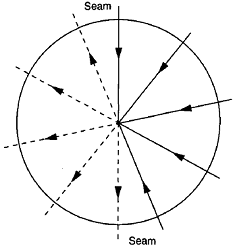
\includegraphics[scale=0.7]{PolarOrbits/planeconfig.png}
\caption{Distribution of the planes for Polar Orbits design.}
\end{center}
\end{figure}

\subsubsection{The Streets of Coverage Method}
This  Street of Coverage Method is obtained from 
\cite{OrbitalMechanics}. As you can see in the figure below,
 the relations between angles seen from different satellites can
 be easily computed. The main variables are the following:
 
\begin{itemize}
\item \begin{equation} N = Number of Satellites 
\end{equation}
\item \begin{equation} S = Separation between satellites
\end{equation}
\item \begin{equation} D = Space between planes [º]
\end{equation}
\item \begin{equation} \varepsilon = Elevation Angle [º]
\end{equation}
\item \begin{equation} \lambda_{street} = Width of the street of coverage[º]
\end{equation}
\item \begin{equation} \lambda_{max} = Maximum Radius of the Footprint[º]
\end{equation}
\end{itemize}
 
\begin{figure}[H]
\begin{center}
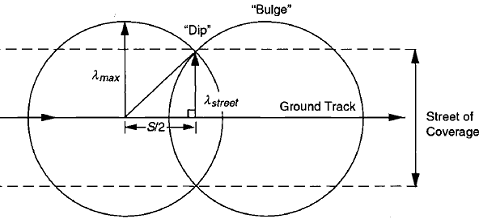
\includegraphics[scale=0.7]{PolarOrbits/planestreet.png}
\caption{Single plain street of coverage. The footprints of the satellites superpose leading to a street.}
\end{center}
\end{figure}

From the figure it can be inferred:

\begin{equation}
S < 2\lambda_{max}
cos(\lambda_{street}) = cos(\lambda_{street})/cos(S/2)
\end{equation}

\begin{figure}[H]
\begin{center}
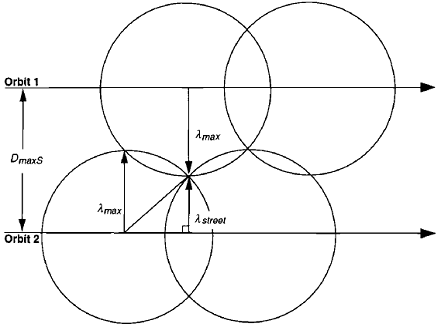
\includegraphics[scale=0.7]{PolarOrbits/planeseps.png}
\caption{Two plains streets of coverage. An optimum phasing needs to be obtained.}
\end{center}
\end{figure}

\begin{equation}
Lenght of the CLTU=10+8\cdot(\frac{Total lenght of the frames+6}{7})
\end{equation} 

%\begin{figure}[H]
%\begin{center}
%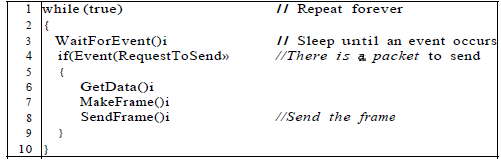
\includegraphics[scale=1]{simplestsender.PNG}
%\caption{Sender algorithm for the simplest protocol.}
%\end{center}
%\end{figure}
%\begin{figure}[H]
%\begin{center}
%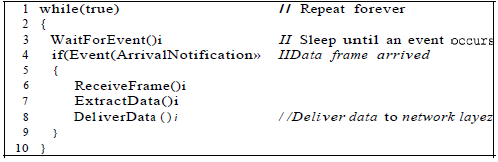
\includegraphics[scale=1]{simplestreceiver.PNG}
%\caption{Receiver algorithm for the simplest protocol.}
%\end{center}
%\end{figure}

\subsection{Results of Streets of Coverage}


\subsection{Example with table}
The standards of the CCSDS will be followed in order to allow interoperability with other satellites such as the one of the client. The CCSDS has developed four protocols for the Data Link Protocol Sublayer of the Data Link Layer\cite{Secretariat2014}:

Paragraph before the table
\begin{table}[H]
\begin{center}
\begin{tabular}{|c|c|}
\hline
\textbf{Protocol}&\textbf{System used for reliability}\\
\hline
TM&Stop-and-Wait Protocol\\
\hline
TC&Type-A: Go-Back-N ARQ, Type-B:Stop-and-Wait Protocol\\
\hline
AOS&Stop-and-Wait Protocol\\
\hline
Proximity-1&Go-Back-N ARQ\\
\hline
\end{tabular}
\caption{Reliability of CCSDS protocols}
\end{center}
\end{table}

According to the table... 

\subsection{Example with equation}
This equation is an example of equation:
 
\begin{equation}
Lenght of the CLTU=10+8\cdot(\frac{Total lenght of the frames+6}{7})
\end{equation} 

The equation is very beautiful
%\bibliographystyle{unsrt}
%\bibliography{forouzan,Secretariat2014,TC,tmsynch,OrbitalMechanics
%\end{document}